\documentclass[12pt]{article}

% Figures
\usepackage{graphicx}
\usepackage{wrapfig}
\graphicspath{{../plots/}{../tikz/}}
\usepackage[section]{placeins}

% fonts and appearance
\usepackage{amsmath, amsfonts, physics, siunitx, fleqn}
\usepackage[american]{babel} 
\usepackage[T1]{fontenc} % improved font encoding
\usepackage{libertine}

% page size and margins
\usepackage{geometry}
\geometry{letterpaper,margin=1in}
\usepackage{fancyhdr}

% better tables
\usepackage{booktabs}
\usepackage{array}
\newcommand{\PreserveBackslash}[1]{\let\temp=\\#1\let\\=\temp}
\newcolumntype{C}[1]{>{\PreserveBackslash\centering}p{#1}}
\newcolumntype{R}[1]{>{\PreserveBackslash\raggedleft}p{#1}}
\newcolumntype{L}[1]{>{\PreserveBackslash\raggedright}p{#1}}

% better lists
\usepackage{enumitem}
\setlist{nosep}

% authors
\usepackage{authblk}
\title{Mainstreaming Adaptive Resilience: how high to elevate a house given multiple PDFs of future flood hazard?}
\author[1]{James Doss-Gollin}
\author[2,3]{Klaus Keller}
\affil[1]{Department of Civil and Environmental Engineering, Rice University}
\affil[2]{Department of Geosciences, the Pennsylvania State University}
\affil[3]{Earth and Environmental Systems Institute, the Pennsylvania State University}
\renewcommand*{\Affilfont}{\normalsize\normalfont}

% ACRONYMS
\usepackage[acronym,nopostdot,nonumberlist,shortcuts,]{glossaries}
\newacronym{bdt}{BDT}{Bayesian decision theory}
\newacronym{bfe}{BFE}{base flood elevation}
\newacronym{dmdu}{DMDU}{decision making under deep uncertainty}
\newacronym{fema}{FEMA}{the Federal Emergency Management Agency}
\newacronym{gcm}{GCM}{general circulation model}
\newacronym{iid}{IID}{independent and identically distributed}
\newacronym{lsl}{LSL}{local mean sea level}
\newacronym{mcmc}{MCMC}{Markov Chain Monte Carlo}
\newacronym{mordm}{MORDM}{multiobjective \gls{rdm}}
\newacronym{pdf}{PDF}{probability density function}
\newacronym{rcp}{RCP}{representative concentration pathway}
\newacronym{rdm}{RDM}{robust decision making}
\newacronym{sow}{SOW}{state of the world}
\newacronym{tc}{TC}{tropical cyclone}

\usepackage{xspace}
\makeatletter
\DeclareRobustCommand\onedot{\futurelet\@let@token\@onedot}
\def\@onedot{\ifx\@let@token.\else.\null\fi\xspace}
\newcommand{\usd}[1]{\SI{#1}[\$]{}}
\def\eg{\emph{e.g}\onedot} \def\Eg{\emph{E.g}\onedot}
\def\ie{\emph{i.e}\onedot} \def\Ie{\emph{I.e}\onedot}
\def\etc{\emph{etc}\onedot} \def\vs{\emph{vs}\onedot}

% use biblatex
\usepackage{csquotes}
\usepackage[
  backend=biber,
  doi=true,
  url=false,
  isbn=false,
  style=authoryear-comp,
  natbib=true,
  backref=false,
  maxbibnames=10,
  maxcitenames=2,
  uniquename=false,
  uniquelist=false,
  sorting=nyt,
]{biblatex}
\renewbibmacro{in:}{}
\AtEveryBibitem{\clearfield{month}\clearfield{day}\clearfield{pages}\clearlist{language}}
\addbibresource{../_bibliography/library.bib}

% load this last
\usepackage[hidelinks]{hyperref}
\usepackage{cleveref}

% up to 1250 words
\begin{document}
\maketitle
\thispagestyle{empty}

\begin{abstract}
    In response to evolving real and perceived flood risk, homeowners, often subsidized by federal and local programs, may invest in building-scale floodproofing measures such as house elevation.
    Federal guidance as to how high to elevate a building relies on floodplain maps that reflect current hazard, suggesting that in regions where flood risk is fast changing, such as along coastlines, incorporating nonstationary flood risk into decision support might lead to dramatically different guidance.
    However, future flood hazard is subject to large and deep uncertainties driven by climate forcings, sea level response, and economics.
    Using a case study of elevating a single home in Norfolk, VA, we first show that decisions tailored to a particular set of assumptions may perform poorly under another.
    This illustrates that even when deep uncertainties are modeled, decision makers must make subjective design choices.
    We present a framework for robust planning under deep uncertainty that transparently maps subjective beliefs to stochastic optimization, and that facilitates computationally cheap \emph{a posteriori} robustness checks to evaluate performance under alternative subjective beliefs.
    We find that ignoring uncertainty between \gls{rcp} scenarios [\texttt{leads to bad outcomes}\ldots].
\end{abstract}
\subsection*{Submission Plan}
We should revisit this!
\begin{enumerate}
    \item Climatic Change
    \item IOP Environmental Research: Infrastructure and Sustainability (new journal)
    \item Earth's Future
    \item Risk analysis
\end{enumerate}
\subsection*{Internal peer review}
\begin{enumerate}
    \item TBD
\end{enumerate}

\clearpage
\section{Introduction}
\begin{enumerate}
    \item Home elevation is an important problem
          \begin{enumerate}
              \item Floodproofing and building-scale vulnerability reduction measures can effectively reduce local flood damages in many contexts \citep{demoel_reducing:2014,deruig_building:2020,kreibich_building:2005,slotter_floodproofing:2020,Rozer:2016dn}
              \item \citet{mobley_mitigation:2020} shows wide potential for elevation to reduce flood losses
              \item \citet{cardenas_elevation:2018} shows that rich Houston residents are already elevating their houses
              \item \citet{aerts_cost:2018} looks at costs of elevation
          \end{enumerate}
    \item Prior studies have illuminated a lot
          \begin{enumerate}
              \item Existing engineering guidance and policy recommend elevating to the \gls{bfe} plus a freeboard \citep{fema_retrofitting:2014,asce_24-14:2015,fema_retrofitting:2014}
              \item \citet{xian_elevation:2017} minimizes discounted expected lifetime costs to show that the optimal elevation can differ substantially from \gls{fema} recommendations
              \item \citet{zarekarizi_suboptimal:2020} expands on this analysis to consider multiple objectives (including those that capture the hard to quantify disruptions of experiencing a flood) and multiple sources of uncertainty (\eg, discount rate, flood probability, and house lifetime)
              \item However, these analyses are silent on the question of how to address deep uncertainties in nonstationary flood hazard
          \end{enumerate}
    \item Multiple \glspl{pdf} present a challenge for coastal adaptation
          \begin{enumerate}
              \item Coastal floods are often decomposed into changes in local sea level \citep{kopp_evolving:2017,kopp_probabilistic:2014,wong_brick0.2:2017} plus storm surge \citep{garner_slrise:2018,cagigal_emulator:2020,rueda_surge:2016}
              \item The choices of \gls{rcp} scenario and model structure matter a lot for sea level \citep{kopp_probabilistic:2014,kopp_evolving:2017,wong_brick0.2:2017,ruckert_coastal:2019,wong_nola:2017}
              \item The choice of statistical representation of storm surge risk matters for future surge risk \citep{wong_nola:2017,wong_structural:2020}
              \item \citet{wong_structural:2020} illustrates the equifinality problem: there may be one or more models that fit the historical data equally well, but give very different results into the future.
          \end{enumerate}
    \item How can robust decision support transparently balance the goals of (i) sampling the tails of plausible future conditions; (ii) integrating information from multiple \gls{rcp} scenarios and models; and (iii) exploiting probabilistic beliefs about the future?
          \begin{enumerate}
              \item \citet{bankes:1993,lempert_shaping:2003,Brown:2012kb} emphasize the importance of using models to explore possibilities and consequences rather than trying to consolidate all information into a single prediction
              \item Exploratory modeling enables the use of non-optimization analytic methods like scenario discovery \citep{kwakkel:2019,lamontagne_discovery:2018}
              \item While we agree with the importance of exploratory modeling, it defers to the decision maker all choices about how to make decisions given a map of possibilities, decisions, and consequences
              \item This motivates a search for ``robust'' approaches, which \citet{herman:2015} reviews how others have conceived of robustness, focusing primarily on identifying the fraction of a parameter space over which some constraints are met
              \item The real world is in a state of ``unknown unknowns'' \citep[level 5 as defined in][fig.~1]{walker_deep:2013} so trying to represent \emph{all} uncertainty is futile; we must make subjective modeling choices and assumptions about what is most important
              \item \citet{mcphail_robustness:2019} elaborates on robustness metrics and their implications
              \item However, these methods are silent on the question of what the distribution or set of \glspl{sow} over which these metrics are calculated should be, and what the robustness of inference is to alternatives.
          \end{enumerate}
\end{enumerate}

In this paper we \ldots

\section{Methods}\label{sec:methods}

We first present a general framework for decision making under uncertainty (\cref{sec:methods-framework}).
This approach is designed for decision problems with a multiplicity of possible futures and outcomes whose likelihood of occurring can be represented quantatively, but necessarily using highly subjective representations.
We then illustrate this method through a didactic case study of deciding if, and how high, to elevate a single house in Norfolk, VA (\cref{sec:methods-case}).
We finally compare our approach to two other robustness metrics (\cref{sec:methods-alternative}).

\subsection{Decision framework}\label{sec:methods-framework}

\begin{figure}
    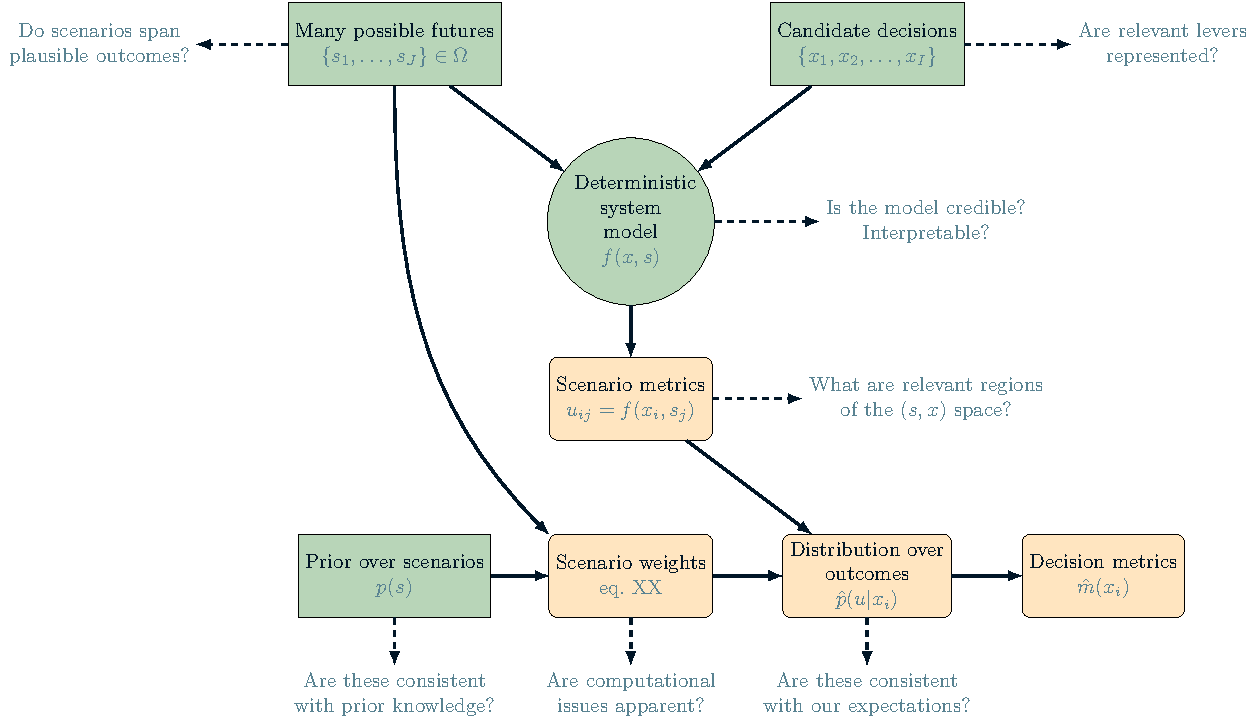
\includegraphics[width=\textwidth]{conceptual.pdf}
    \caption{
        Schematic of general decision framework and definitions.
        Nodes in green are modeling inputs, those in yellow are derived quantities, and those in gray describe opportunities for iterative model critique and examination to support decision-making.
    }\label{fig:framework}
\end{figure}
Our decision framework, illustrated in \cref{fig:framework}, draws from three main bodies of literature.

First, the literature on \gls{dmdu} emphasizes the importance of identifying decisions that perform well over a wide range of possible futures.
Exploratory modeling can demonstrate the existence of particular outcomes, generate hypotheses, build qualitative insight, and identify scenarios worthy of further study \citep[see][]{bankes:1993}.
Exploring many possible futures is particularly important when facing deep and epistemic uncertainties \citep{lempert_shaping:2003,wong_nola:2017,oddo_coastal:2017}
Many tools used for \gls{dmdu} including decision scaling \citep{Brown:2012kb}, robust decision making \citep{lempert:2007,kasprzyk:2013,kasprzyk_denovo:2012}, sensitivity analysis \citep{saltelli_comment:2019}, and scenario discovery \citep{kwakkel:2019,lamontagne_discovery:2018}, build on the idea of exploratory modeling, and we incorporate this philosophy into our approach.



The observation that many of these mechanisms cannot be represented by a single objective \gls{pdf} has motivated many criticisms of the application of \gls{bdt} to planning problems.
Yet \gls{bdt} was conceived as a calculus for reasoning rather than for identifying objective truth; \citeauthor{definetti_probability:1972} often said that ``probability does not exist'' \citeyear{definetti_probability:1972}.
\citet{savage:1954} and \citet{ramsey_probability:2016}, among others, also viewed probability as ``subjective,'' representing the state of belief of the decision-maker.
The famous phrase ``all models are wrong, but some are useful'' \citep[generally attributed to][]{box:1976} also suggests that probability distributions and predictions ought to be viewed subjectively.
More recent discussions of Bayesian philosophy \citep{jaynes_probability:2003,McElreath:2016vu,Gelman:2014tc,bernardo_bayesian:1994} also emphasize a philosophical view of probability as a language with which to reason about the unknown rather than a statement of objective truth \citep[see][for a thorough discussion of Bayesian philosophy]{gelman_philosophy:2013}.
Although the true data generating process is not known and inference should not be represented as objective truth, probability gives a transparent and consistent language for reasoning about uncertainty.

Since modeling assumptions cannot overcome epistemic uncertainty, even with better models and more data, we draw from the literature on statistical model selection in the $\mathcal{M}$-open setting, which provides a theoretical background for choosing between models when the true data generating process is not among the models considered \citep[see][]{Piironen:2017eh}.
Often, combining inferences from multiple models is more effective than seeking a single ``best'' model \citep{Yao:2018bu}.
More fundamentally, this literature emphasizes the importance of iteratively building models, simulating the consequences of those models, and critiquing them \citep{gelman_workflow:2020}.
Since, by definition, models are not ``true,'' this iterative workflow aims to identify models that are useful and promote a dialog amongst stakeholders \citep{gelman_philosophy:2013}.

\subsubsection{Exploratory modeling}

Following \citet{mcphail_robustness:2019}, we consider a set of decisions $x_1, \ldots, x_m \in \mathcal{X}$ as well as a set of plausible future conditions (scenarios) $s_1, \ldots, s_n \in \Omega$.
We refer to $\mathcal{X}$ as the decision space and $\Omega$ as the event space.
To evaluate a given decision $x_i$, we use an arbitrary system model $f: \mathcal{X} \times \mathcal{S} \rightarrow \mathcal{U}$ to compute a scalar or vector performance metric $u \in \mathcal{U}$ for each scenario.
We define the performance of the $i$th decision on the $j$th scenario as $u_{ij} = f(x_i, s_j)$ and call the $u_{ij}$ ``scenario metrics.''
The full set $u_{i1}, \ldots, u_{in}$ can be used in a fully exploratory context \citep[\eg, scenario discovery;][]{kwakkel:2019,lamontagne_discovery:2018} to identify the conditions under which a given decision $x_i$ performs well or poorly.
These consequences can also be shared with stakeholders to improve the model, assess the completeness of scenarios considered, or expand the decision set.

\subsubsection{Probabilistic modeling}

If the decision space is small, then exploratory modeling may provide sufficient information for decision making.
However, as the decision space grows large it becomes helpful to develop ``decision metrics'' $\hat{m}(x_i)$, that summarize performance across all scenarios.

A general approach is define the decision metrics as a weighted sum of the scenario metrics: $\hat{m}(x_i) = \sum_{j=1}^n w_j u_{ij}$.
Many commonly used heuristics can be described using this framework.
In the most extreme case, maximum and minimum metrics set all $w_j$ but one to zero, conveying information only about worst-case performance.
In the other extreme, setting $wj \propto 1$ conveys information about all scenarios, but is sensitive to the set of scenarios considered.
A more stable alternative is to set the weights using a \gls{pdf} to describe subjective belief about the likelihood of each scenario, $p_\text{belief}(\Sigma)$, and then to use this \gls{pdf} to set the scenario weights.
Given a probabilistic belief model on the sample space $p_\text{belief}(x)$, the weight assigned to the $i$th scenario is
\begin{equation}\label{eq:scenario-weight}
    w_i \propto \frac{p_\text{belief}(x_i)}{\hat{p}_\text{sampling}(x_i)},
\end{equation}
where $\hat{p}_\text{sampling}$ is the sampling distribution estimated using, \eg, kernel density estimation.
\Cref{eq:scenario-weight} is equivalent to the definition of rejection sampling, except that instead of accepting draws from a proposal distribution (here $\hat{p}_\text{sampling}$) with probability $w_i$ to generate \gls{iid} draws from the target distribution (here $p_\text{belief}$), we retain and weight all scenarios.

Setting the weights from a \gls{pdf} has several advantages:
\begin{enumerate}
    \item we gain a formal justification for reasoning about the \emph{distribution} of outcomes, $\hat{p}(y | x_i)$, rather than merely a \emph{set} of possible outcomes;
    \item the decision metric $\hat{m}(x_i)$ is stable if the sampling distribution is changed (\eg, if new scenarios are added); and
    \item the subjective assumption on $p_\text{belief}$ is highly transparent and can be critiqued, \eg by interpreting $p_\text{belief}$ as a prior in a Bayesian framework \citep{Gelman:2014tc,McElreath:2016vu} and conducting prior predictive checks to identify, improve, and communicate the joint implications of the model and prior \citep[see][section 2.4]{gelman_workflow:2020}.
\end{enumerate}
Since the choice of \gls{pdf} to represent the analyst's subjective belief about the likelihood of different scenario is necessarily subjective, it is advisable to formulate several plausible \glspl{pdf} and compare performance across them.
The computational effort required for this is quite low: using a different numerator in \cref{eq:scenario-weight}, the weights assigned to each scenario are updated, but the system model does not need to be re-run.
Thus, answering the question ``what does the distribution''
We illustrate this approach in the house elevation case study (\cref{sec:methods-case}).

\subsubsection{Iterative model critique and robustness checks}

Drawing from iterative model building philosophies of the statistical and decision science communities, the fundamental goal of our decision analysis is to use a model to transparently examine the implications of various assumptions.
\Cref{fig:framework} illustrates several opportunities for iterative validation, critique, and improvement of the full decision problem.



We next turn to the problem posed by the intrinsically subjective choice of $p_\text{belief}$.
The \gls{dmdu} literature emphasizes the importance of identifying decisions that are robust, often defined as trading some performance in the most likely scenario for performance in other plausible futures.
In

Since our $p_\text{belief}$ is subjective, we define robustness in terms of alternative beliefs that other reasonable analysts might hold.
Obviously the full space of all possible beliefs cannot be computed any more than the full set of all possible models or datasets or problem framings can be defined, and so such a comparison is necessarily qualitative.
However, many alternative beliefs can easily be computed because only the $w_i$ need to be recomputed to evaluate performance under another belief; the $y_{ij}$ are unchanged and thus, the model does not need to be re-run.

\subsection{Case study: house elevation}\label{sec:methods-case}

\begin{table}
    \centering
    \begin{tabular}{llr}
        \toprule
        Uncertainty           & Treatment                                    & Discussed in                      \\
        \midrule
        Sea Level             & Deep uncertainty: 4 \acrshort{rcp} scenarios & \cref{sec:methods-lsl}            \\
        Storm Surge           & Parametric uncertainty                       & \cref{sec:methods-surge}          \\
        Discount Rate         & Fixed constant                               & \cref{sec:methods-cost}           \\
        Planning Horizon      & Fixed constant                               & \cref{sec:methods-cost}           \\
        Depth-Damage Function & Deterministic and known                      & \cref{sec:methods-cost-damage}    \\
        Cost of Elevation     & Deterministic and known                      & \cref{sec:methods-cost-elevation} \\
        \bottomrule
    \end{tabular}
    \caption{
        Treatment of potential sources of uncertainty.
        As indicated, strong assumptions are made as to some potential sources of uncertainty in order to maintain interpretability of findings.
    }\label{sec:tab-uncertainties}
\end{table}

\subsection{Sea Level}\label{sec:methods-lsl}

We use BRICK \citep{wong_brick0.2:2017} simulations from \citet{ruckert_coastal:2019}, which is sufficient to include both model structure uncertainty (fast or slow dynamics) and human factors (\gls{rcp} 2.6, 4.5, 6.0, or 8.5).

\subsection{Storm Surge}\label{sec:methods-surge}

Define $\mu^*(t)=\mu_0 + \beta \qty(t-t_0)$, where $t_0$ is 2020. Then $y'(t) \sim \text{GEV}(\mu^*(t), \rho \mu^*(t), \xi)$, where $\rho$ is a coefficient of variation. We can put together a single model for storm surge with informative priors, and note that there are other models that we could look at in future work.

\subsection{Costs}\label{sec:methods-cost}

Our objective is to minimize discounted total costs (initial cost of construction plus expected future damages), taken as a weighted average over $N$ modeled realizations of the future, over a fixed 50 year period.
$$\min C_e(\Delta h) + \sum_{i=1}^N \sum_{t=2020}^{2070} \gamma_t w_i D(y_{i,t}, \Delta h) $$
where $D$ is the loss or damage function and $w_i$ is a weight applied to the $i$th scenario such that $\sum_{i=1}^N w_i = 1$.
We can keep the discount rate fixed for concision: $\gamma_t = 0.97^t$ is a 3\% rate -- we can vary this number but let's keep it simple.

\subsubsection{Flood Damage}\label{sec:methods-cost-damage}

Flood damage as \citet{zarekarizi_suboptimal:2020}.

\subsubsection{Elevation Cost}\label{sec:methods-cost-elevation}
Elevation Cost as \citet{zarekarizi_suboptimal:2020}.

\subsubsection{Belief model}

\begin{table}
    \centering
    \footnotesize
    \begin{tabular}{L{1in}L{0.75in}L{0.5in}L{3.5in}}
        \toprule
        Variable                     &
        distribution                 &
        University                   &
        Discussion                                                                                                                                           \\
        \midrule
        LSL in 2100                  &
        $\mathcal{N}(1, 1)$          &
        \si{m}                       &
        Express a belief about sea level in 2100, which is well studied, and treat all scenarios with the same $\overline{y}_{2100}$ as equally likely       \\
                                     &
        $\mathcal{N}(1.25, 1.25)$    &
                                     &
        Different prior belief                                                                                                                               \\
        RCP scenario                 &
        $\mathcal{N}(4.5, 1.5)$      &
        \si{\watt\per\meter\squared} &
        Express a prior belief that RCP 4.5 is most likely. This amounts to treating each scenario as IID given the RCP scenario and then weighting the PDFs \\
                                     &
        $\mathcal{N}(6.0, 1.5)$      &
                                     &
        As above, but belief that RCP 6 is most likely.                                                                                                      \\
        Uniform                      &
        $w_i \propto 1$              &
                                     &
        Treat all scenarios as equally likely, implying that $\hat{p}_\text{sampling} = p_\text{belief}$.                                                    \\
        \bottomrule
    \end{tabular}
    \caption{Prior beliefs}
\end{table}

\subsection{Decision Model}\label{sec:methods-decision}

\begin{enumerate}
    \item We sample $N$ scenarios from the set of plausible future outcomes, consistent with ideals of exploratory modeling \citep{bankes:1993} \citep[indeed we can use samples for scenario discovery;][]{kwakkel:2019}
    \item If $w_i = \frac{1}{N} \, \forall \, i \in 1, \ldots, N$ then all scenarios are treated equally; this is what is typically used in robustness metrics (though instead of a continuous objective function a binary satisficing constraint is often used; see \citealt{herman:2015} or \citealt{kwakkel:2019})
    \item However, this reveals a tension: we want to \emph{explore} highly unlikely but theoretically possible trajectories to understand their consequences, but we don't want extremely unlikely scenarios to dominate our decision
    \item To see how this works in high dimensions, if we make the (admittedly silly) assumption that the true distribution is uniform within a sphere and we sample the enclosing hypercube, the fraction of samples that are likely is
          $$ \frac{\pi^\frac{n}{2}}{\Gamma(\frac{n}{2} + 1)} \frac{1}{2^n}$$
          which if $n=7$ is about 3.7\%. (This is just an illustration of how high dimensions work)
    \item Similarly, we want decisions that do not change drastically if we change the sampling dimension. For example, if we explore \gls{rcp} 2.6, 4.5, 6, and 8.5, and then we consider \gls{rcp} 4.6 (just like 4.5 but very very slightly modified), our decisions should not change dramatically
    \item We therefore have two key steps:
          \begin{enumerate}
              \item A function $g: \mathcal{X} \rightarrow \mathcal{Z}$ that maps a realization of the future $x \in \mathcal{X}$ to a low-dimension representation $z \in \mathcal{Z}$. In our case, $\mathcal{Z}$ is just the sea level in 2100
              \item A subjective joint probability distribution over $\mathcal{Z}$: $p(\mathcal{Z})$
          \end{enumerate}
    \item This is conceptually similar to the approach of \citet{garner_slrise:2018}
    \item the steps are thus:
          \begin{enumerate}
              \item Start with a set of $N$ realizations of the future
              \item Define a low dimension space $\mathcal{Z}$ and a subjective probability belief $p(\mathcal{Z})$
              \item Compute the sampling distribution $p_\text{sampling}(\mathcal{Z})$ using, \eg, kernel density estimation
              \item Assign each realization a weight $w_i = \frac{p(\mathcal{Z})}{p_\text{sampling}(\mathcal{Z})}$.
              \item Run the optimization
              \item Optionally (but highly encouraged!), coonduct robustness checks by altering $p_\text{sampling}(\mathcal{Z})$ and recomputing expected outcomes. Since outcomes have already been calculated for each realization $x_i \forall i=1,\ldots,N$, outcomes can be recomputed with new weights with no need to run any additional calculations
          \end{enumerate}
\end{enumerate}

\subsection{Alternative decision frameworks}\label{sec:methods-alternative}

\subsubsection{Minimax regret}

\subsubsection{Hypervolume satisficing}

We follow \citet{zarekarizi_suboptimal:2020} exactly.

\section{Results}

\begin{enumerate}
    \item Show a scenario map, fixing $x_i$ to be FEMA recommendation (elevate to the 100 year flood estimated from a historic GEV plus freeboard). The two axes can represent mean sea level in 2070 and the 99th percentile of storm surge in 2070. Each dot can be a scenario.
\end{enumerate}

\section{Discussion}

\begin{enumerate}
    \item There are other objectives that might be useful for real-world decision support
          \begin{enumerate}
              \item We focused on cost minimization for simplicity but practical decision support might consider many objectives
              \item Real people might care about uncertainty (risk aversion), probability of experiencing flooding at all (disruptions are hard to quantify), usable space created under the house,
          \end{enumerate}
    \item Similarly, there are other considerations and sources of uncertainty that we could incorporate
          \begin{enumerate}
              \item Damage functions, cost of construction, house lifespan, discount rate, \etc
              \item We could have a sequential decision with learning (about sea level rise, cost of construction, and more)
              \item Data on cost of elevation and depth-damage is insufficiently recent, localized, and accurate.
              \item Optimization is for a single house, not many different structures and locations.
          \end{enumerate}
    \item Comparison to other definitions and understandings of robustness
          \begin{enumerate}
              \item One could pick a single sea level rise time series and optimize for it, then look at how well this meets some satisficing criteria for other plausible sea level rise time series. But how do you pick your best guess? How do you measure satisficing? How do you sample alternative SOWs against which to calculate this satisficing?
              \item One could do full stochastic optimization, \ie Bayesian Decision Theory. But how do you pick the ``objective'' probability distribution to use? In practice this often means choosing a model and RCP scenario and then drawing scenario-conditional samples.
              \item Our approach draws from both perspectives: we sample across deep uncertainties (like RCP scenario) using a subjective probability distribution, then assess robustness by quantifying how well this decision performs if other subjective distributions are used.
          \end{enumerate}
    \item There are links to a literature on model averaging
          \begin{enumerate}
              \item Stacking \citep{Yao:2018bu}
              \item Bayesian model averaging \citep{massoud_bma:2020,bhat_bma:2011}
              \item Importantly, we are not attempting to use historical data to weight models, but rather using transparent assumptions about the future to weight realizations of models.
          \end{enumerate}
    \item Our belief model $g : \mathcal{X} \rightarrow \mathcal{Z}$ is limited because $\mathcal{Z} \in \mathbb{R}$, but other measures beyond sea level in 2100 might be useful. For our approach to be valid, we implicitly assume that all candidate realizations are equally likely, conditional on the information contained in $\mathcal{Z}$. In practice we might wish to encode beliefs about future greenhouse forcing, temperature, sea level response to temperature, or other measures.
    \item The benefits of this approach:
          \begin{enumerate}
              \item A goal is to make -- intrinsically flawed and subjective -- modeling choices as transparent as possible. Since we can't be right, we should make it as easy as possible for others to understand and critique our assumptions
              \item Because of how we weight realizations of the future, you can apply a different weighting function and immediately assess performance. Thus qualitative and quantitative sensitivity analyses are simple.
              \item Of course the choice of $p(\mathcal{Z})$ is subjective, but so is every other aspect of how we frame the problem. Modeling is intrinsically subjective. The idea of embracing subjective choices -- and making them explicit and open to critique -- draws heavily from philosophies of iterative workflow in statistics \citep{box:1976,gelman_workflow:2020,gelman_philosophy:2013}.
              \item This approach can be used in a multiobjective context and is an alternative way to measure robustness in \gls{rdm} and \gls{mordm}
          \end{enumerate}
    \item This approach can be used in many other contexts
          \begin{enumerate}
              \item Stormwater management \citep{sharma_stormwater:2021,lopez-cantu:2018}
              \item Levee heightening \citep{garner_slrise:2018,oddo_coastal:2017,vandantzig_dike:1956}
          \end{enumerate}
\end{enumerate}

\section{End Matter}

\subsection{Acknowledgements}

\begin{enumerate}
    \item MARISA (details!) for JDG funding
    \item PSIRC (details!) for JDG funding
    \item Tor Erlend Fjelde for helpful advice on implementing the GEV prior using \texttt{Turing.jl}.
\end{enumerate}

\subsection{Author Contributions}

See journal requirements and format

\subsection{Supplementary Materials}

\begin{enumerate}
    \item Supplementary figures and analysis online
    \item Link to live repository on GitHub
    \item Link to code DOI on Zenodo
\end{enumerate}

\printbibliography
\end{document}
